\chapter{Đọc thêm 2: Think Stats -- Phân tích dữ liệu khám phá bằng Python (Mục 5.2--5.4)}
\label{ch:M2L2-reading2}

% Nguồn: Downey, Allen B. \emph{Think Stats: Exploratory Data Analysis in Python}. Version 2.2.0, Green Tea Press, 2014. https://greenteapress.com/thinkstats2/thinkstats2.pdf
% Phần cần đọc: Mục 5.2--5.4 (tr. 60--66, ~15 phút)
% Nội dung bắt buộc đọc: được kiểm tra trong mọi bài đánh giá (kể cả Quiz).

\section{Thông tin nguồn}

\begin{itemize}
  \item \textbf{Nguồn:} Downey, Allen B. \emph{Think Stats: Exploratory Data Analysis in Python}. Version 2.2.0, Green Tea Press, 2014. \url{https://greenteapress.com/thinkstats2/thinkstats2.pdf}
  \item \textbf{Phần cần đọc:} Mục 5.2--5.4 (tr. 60--66, ~15 phút)
\end{itemize}

> Nguồn: \texttt{thinkstats2.pdf} (Downey) > Phạm vi: Mục 5.2 - 5.4

% [PDF p.80 | in p.60]
\subsection*{5.2 Phân phối chuẩn}
\addcontentsline{toc}{subsection}{5.2 Phân phối chuẩn}

Phân phối chuẩn (normal distribution), còn được gọi là phân phối Gaussian (Gaussian), thường được sử dụng vì nó mô tả nhiều hiện tượng, ít nhất là ở mức xấp xỉ. Hóa ra có một lý do chính đáng cho sự phổ biến của nó, điều mà chúng ta sẽ tìm hiểu ở Mục 14.4.

Phân phối chuẩn được đặc trưng bởi hai tham số: giá trị trung bình (mean), $\mu$, và độ lệch chuẩn (standard deviation) $\sigma$. Phân phối chuẩn với $\mu = 0$ và $\sigma = 1$ được gọi là phân phối chuẩn tắc (standard normal distribution). Hàm phân phối tích lũy (CDF) của nó được định nghĩa bởi một tích phân không có dạng đóng, nhưng có các thuật toán để tính toán nó một cách hiệu quả. Một trong số đó được cung cấp bởi SciPy: \texttt{scipy.stats.norm} là một đối tượng đại diện cho một phân phối chuẩn; nó cung cấp một phương thức, \texttt{cdf}, để tính toán CDF của phân phối chuẩn tắc:

\begin{lstlisting}[language=Python,escapeinside={(*@}{@*)}]
>>> import scipy.stats
>>> scipy.stats.norm.cdf(0)
0.5
\end{lstlisting}

Kết quả này là chính xác: trung vị (median) của phân phối chuẩn tắc là 0 (giống với giá trị trung bình), và một nửa các giá trị nằm dưới trung vị, vì vậy CDF(0) là 0.5.

% [PDF p.81 | in p.61]
\begin{figure}[H]
\centering
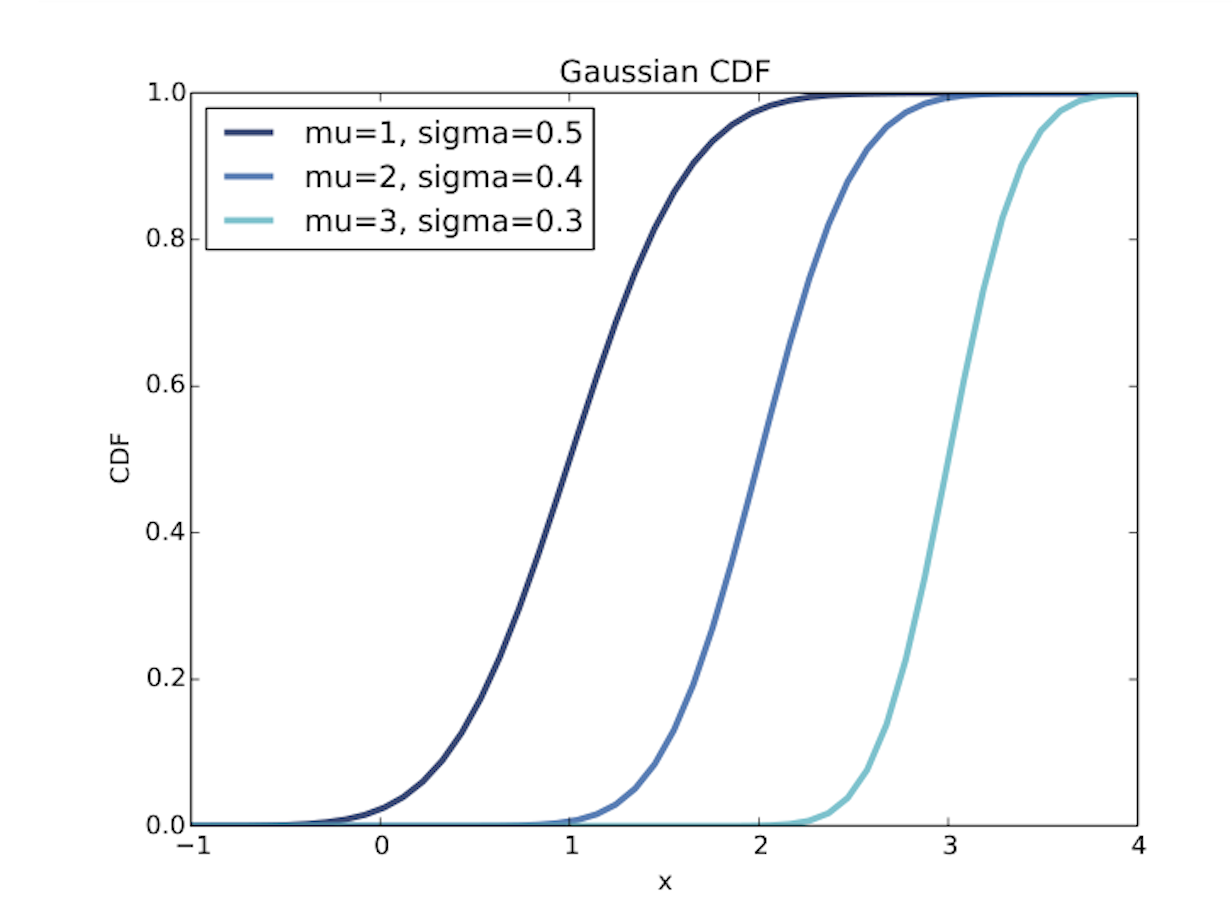
\includegraphics[width=\linewidth,height=0.6\textheight,keepaspectratio]{gfx/m2l2_thinkstats_fig5-3_normal_cdf_params.png}
\par\smallskip{\small \textbf{Hình 5.3:} CDF của các phân phối chuẩn với một loạt các tham số.}
\end{figure}

\texttt{norm.cdf} nhận các tham số tùy chọn: \texttt{loc}, tham số xác định giá trị trung bình, và \texttt{scale}, tham số xác định độ lệch chuẩn.

\texttt{thinkstats2} làm cho hàm này dễ sử dụng hơn một chút bằng cách cung cấp \texttt{EvalNormalCdf}, hàm này nhận các tham số \texttt{mu} và \texttt{sigma} và tính toán CDF tại \texttt{x}:

\begin{lstlisting}[language=Python,escapeinside={(*@}{@*)}]
def EvalNormalCdf(x, mu=0, sigma=1):
    return scipy.stats.norm.cdf(x, loc=mu, scale=sigma)
\end{lstlisting}

Hình 5.3 cho thấy các CDF đối với các phân phối chuẩn với một loạt các tham số. Hình dạng sigmoid của các đường cong này là một đặc điểm dễ nhận biết của phân phối chuẩn.

Trong chương trước, chúng ta đã xem xét phân phối của cân nặng sơ sinh trong NSFG. Hình 5.4 cho thấy CDF thực nghiệm của cân nặng đối với tất cả trẻ sinh sống (live births) và CDF của một phân phối chuẩn có cùng giá trị trung bình và phương sai.

Phân phối chuẩn là một mô hình tốt cho tập dữ liệu này, vì vậy nếu chúng ta tóm tắt phân phối bằng các tham số $\mu = 7.28$ và $\sigma = 1.24$, sai số thu được (sự khác biệt giữa mô hình và dữ liệu) là nhỏ.

Dưới bách phân vị (percentile) thứ 10 có sự sai lệch giữa dữ liệu và mô hình; có nhiều em bé nhẹ cân hơn so với những gì chúng ta kỳ vọng ở một phân phối chuẩn. Nếu chúng ta đặc biệt quan tâm đến trẻ sinh non (preterm babies), điều quan trọng là...

% [PDF p.82 | in p.62]
\begin{figure}[H]
\centering
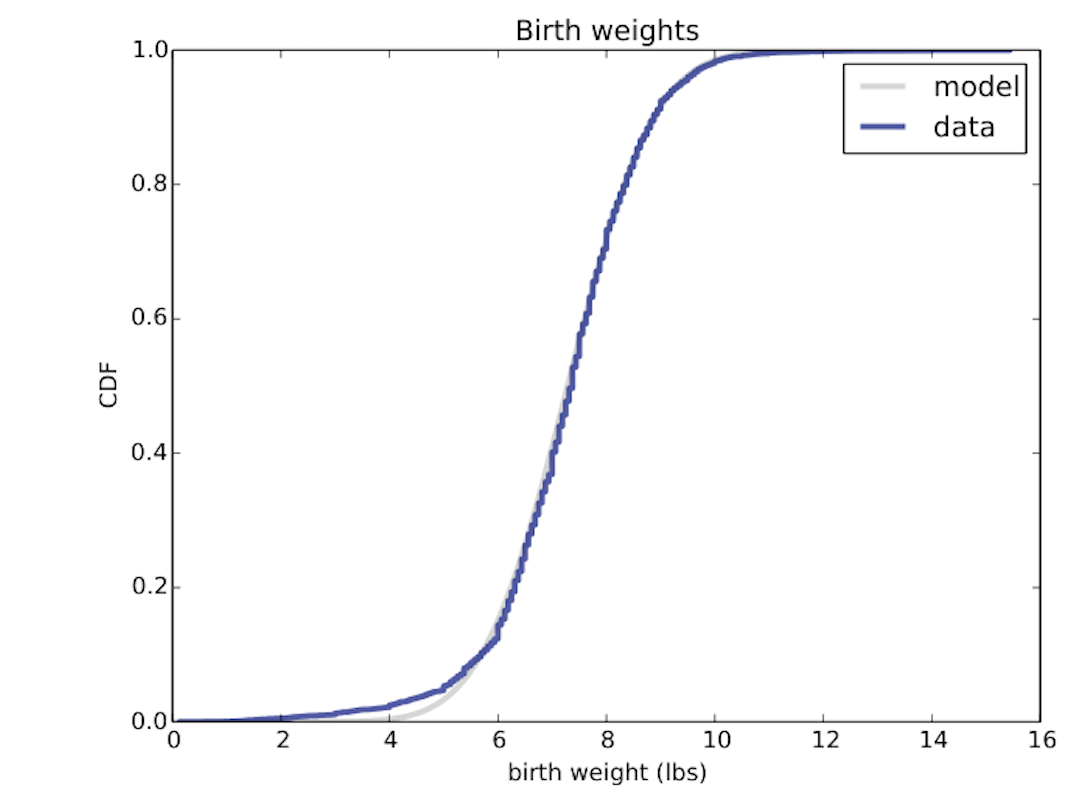
\includegraphics[width=\linewidth,height=0.6\textheight,keepaspectratio]{gfx/m2l2_thinkstats_fig5-4_birth_weights_cdf.png}
\par\smallskip{\small \textbf{Hình 5.4:} CDF của cân nặng sơ sinh với mô hình chuẩn.}
\end{figure}

...phải hiểu đúng phần này của phân phối, vì vậy có thể sẽ không phù hợp nếu sử dụng mô hình chuẩn.

\subsection*{5.3 Biểu đồ xác suất chuẩn}
\addcontentsline{toc}{subsection}{5.3 Biểu đồ xác suất chuẩn}

Đối với phân phối mũ, và một vài phân phối khác, có những phép biến đổi đơn giản mà chúng ta có thể sử dụng để kiểm tra xem một phân phối giải tích (analytic distribution) có phải là một mô hình tốt cho một tập dữ liệu hay không.

Đối với phân phối chuẩn, không có phép biến đổi nào như vậy, nhưng có một giải pháp thay thế được gọi là biểu đồ xác suất chuẩn (normal probability plot). Có hai cách để tạo một biểu đồ xác suất chuẩn: cách khó và cách dễ. Nếu bạn quan tâm đến cách khó, bạn có thể đọc về nó tại \url{https://en.wikipedia.org/wiki/Normal_probability_plot}. Đây là cách dễ:

\begin{enumerate}
  \item Sắp xếp các giá trị trong mẫu.
  \item Từ một phân phối chuẩn tắc ($\mu = 0$ và $\sigma = 1$), tạo một mẫu ngẫu nhiên có cùng kích thước với mẫu, và sắp xếp nó.
  \item Vẽ đồ thị các giá trị đã sắp xếp từ mẫu so với các giá trị ngẫu nhiên.
% [PDF p.83 | in p.63]
\end{enumerate}
\begin{figure}[H]
\centering
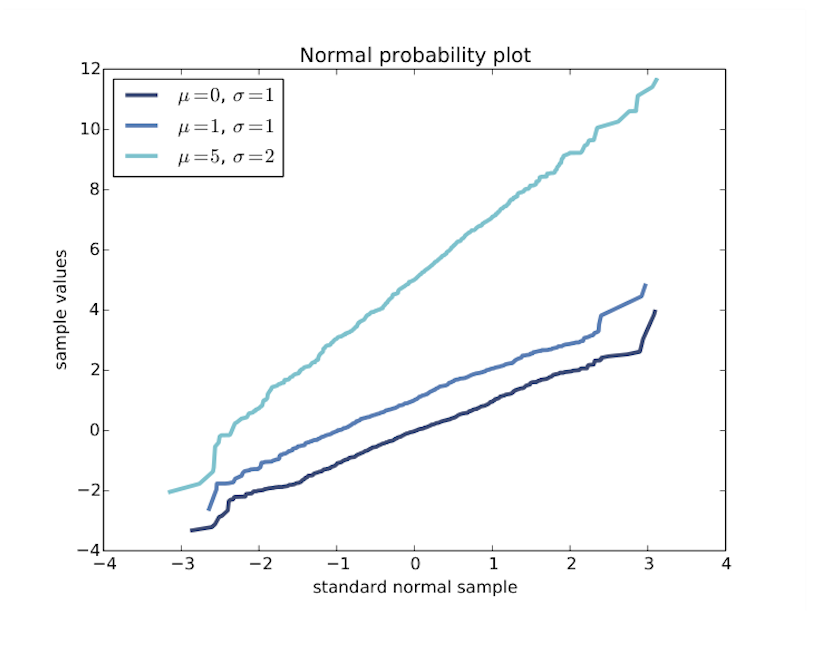
\includegraphics[width=\linewidth,height=0.6\textheight,keepaspectratio]{gfx/m2l2_thinkstats_fig5-5_normal_prob_plot_samples.png}
\par\smallskip{\small \textbf{Hình 5.5:} Biểu đồ xác suất chuẩn cho các mẫu ngẫu nhiên từ các phân phối chuẩn.}
\end{figure}

Nếu phân phối của mẫu gần với phân phối chuẩn, kết quả là một đường thẳng với điểm giao cắt (intercept) là \texttt{mu} và độ dốc (slope) là \texttt{sigma}.

\texttt{thinkstats2} cung cấp \texttt{NormalProbability}, hàm này nhận một mẫu và trả về hai mảng NumPy:

\begin{lstlisting}[language=Python,escapeinside={(*@}{@*)}]
xs, ys = thinkstats2.NormalProbability(sample)
\end{lstlisting}

\texttt{ys} chứa các giá trị đã sắp xếp từ \texttt{sample}; \texttt{xs} chứa các giá trị ngẫu nhiên từ phân phối chuẩn tắc.

Để kiểm tra \texttt{NormalProbability}, tôi đã tạo một số mẫu giả thực chất được rút ra từ các phân phối chuẩn với nhiều tham số khác nhau. Hình 5.5 cho thấy kết quả. Các đường xấp xỉ thẳng, với các giá trị ở các phần đuôi lệch nhiều hơn so với các giá trị gần giá trị trung bình.

Bây giờ hãy thử với dữ liệu thực. Dưới đây là đoạn mã để tạo một biểu đồ xác suất chuẩn cho dữ liệu cân nặng sơ sinh từ phần trước. Nó vẽ một đường màu xám đại diện cho mô hình và một đường màu xanh lam đại diện cho dữ liệu.

\begin{lstlisting}[language=Python,escapeinside={(*@}{@*)}]
def MakeNormalPlot(weights):
    mean = weights.mean()
    std = weights.std()
    xs = [-4, 4]
    fxs, fys = thinkstats2.FitLine(xs, inter=mean, slope=std)
\end{lstlisting}

% [PDF p.84 | in p.64]
\begin{figure}[H]
\centering
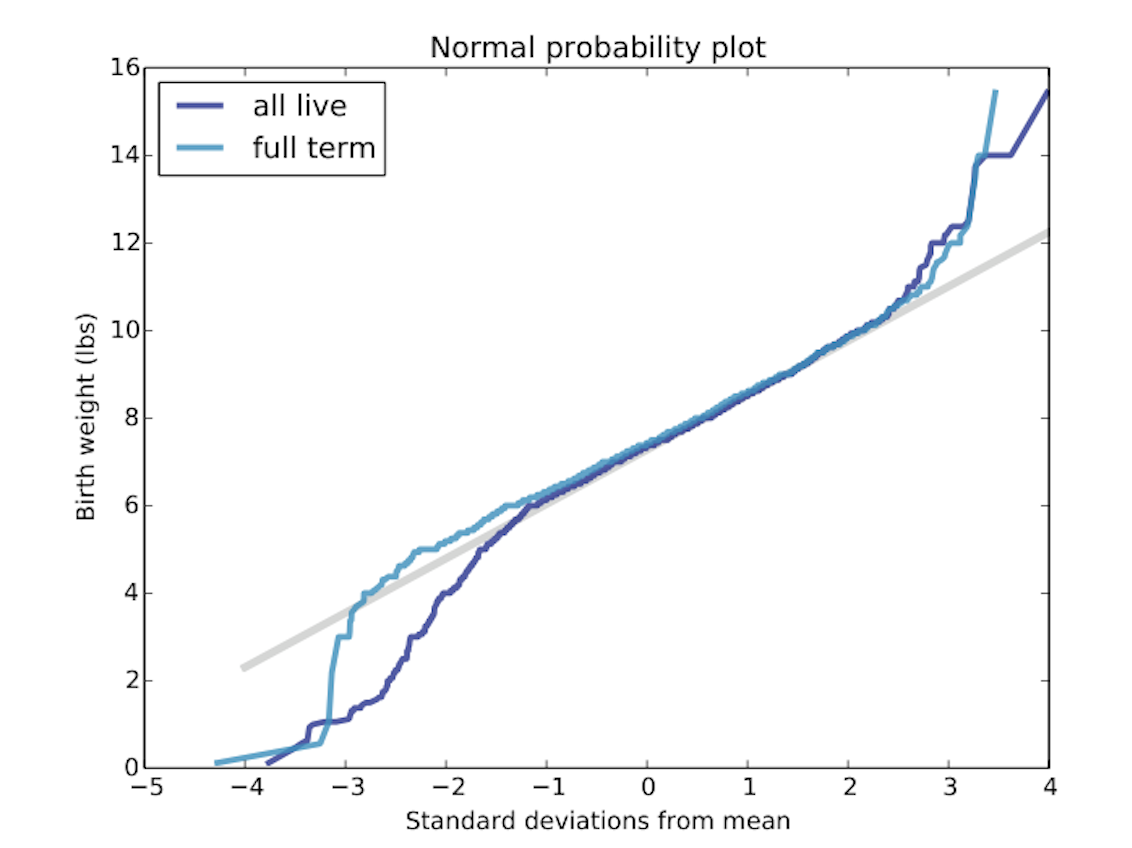
\includegraphics[width=\linewidth,height=0.6\textheight,keepaspectratio]{gfx/m2l2_thinkstats_fig5-6_birth_weights_normal_plot.png}
\par\smallskip{\small \textbf{Hình 5.6:} Biểu đồ xác suất chuẩn của cân nặng sơ sinh.}
\end{figure}

\begin{lstlisting}[language=Python,escapeinside={(*@}{@*)}]
    thinkplot.Plot(fxs, fys, color='gray', label='model')
    xs, ys = thinkstats2.NormalProbability(weights)
    thinkplot.Plot(xs, ys, label='birth weights')
\end{lstlisting}

\texttt{weights} là một Series pandas chứa cân nặng sơ sinh; \texttt{mean} và \texttt{std} là giá trị trung bình và độ lệch chuẩn.

\texttt{FitLine} nhận một chuỗi \texttt{xs}, một điểm giao cắt và một độ dốc; nó trả về \texttt{xs} và \texttt{ys} đại diện cho một đường thẳng với các tham số đã cho, được tính toán tại các giá trị trong \texttt{xs}.

\texttt{NormalProbability} trả về \texttt{xs} và \texttt{ys} chứa các giá trị từ phân phối chuẩn tắc và các giá trị từ \texttt{weights}. Nếu phân phối của \texttt{weights} là phân phối chuẩn, dữ liệu sẽ khớp với mô hình.

Hình 5.6 cho thấy kết quả đối với tất cả trẻ sinh sống, và cả đối với trẻ sinh đủ tháng (thời gian mang thai (pregnancy length) lớn hơn 36 tuần). Cả hai đường cong đều khớp với mô hình ở gần giá trị trung bình và lệch ở các phần đuôi. Những em bé nặng nhất thì nặng hơn so với những gì mô hình kỳ vọng, và những em bé nhẹ nhất thì nhẹ hơn.

Khi chúng ta chỉ chọn các ca sinh đủ tháng, chúng ta loại bỏ một số mức cân nặng nhẹ nhất, điều này làm giảm sự sai lệch ở phần đuôi dưới của phân phối.

Biểu đồ này gợi ý rằng mô hình chuẩn mô tả tốt phân phối...

% [PDF p.85 | in p.65]
\begin{figure}[H]
\centering
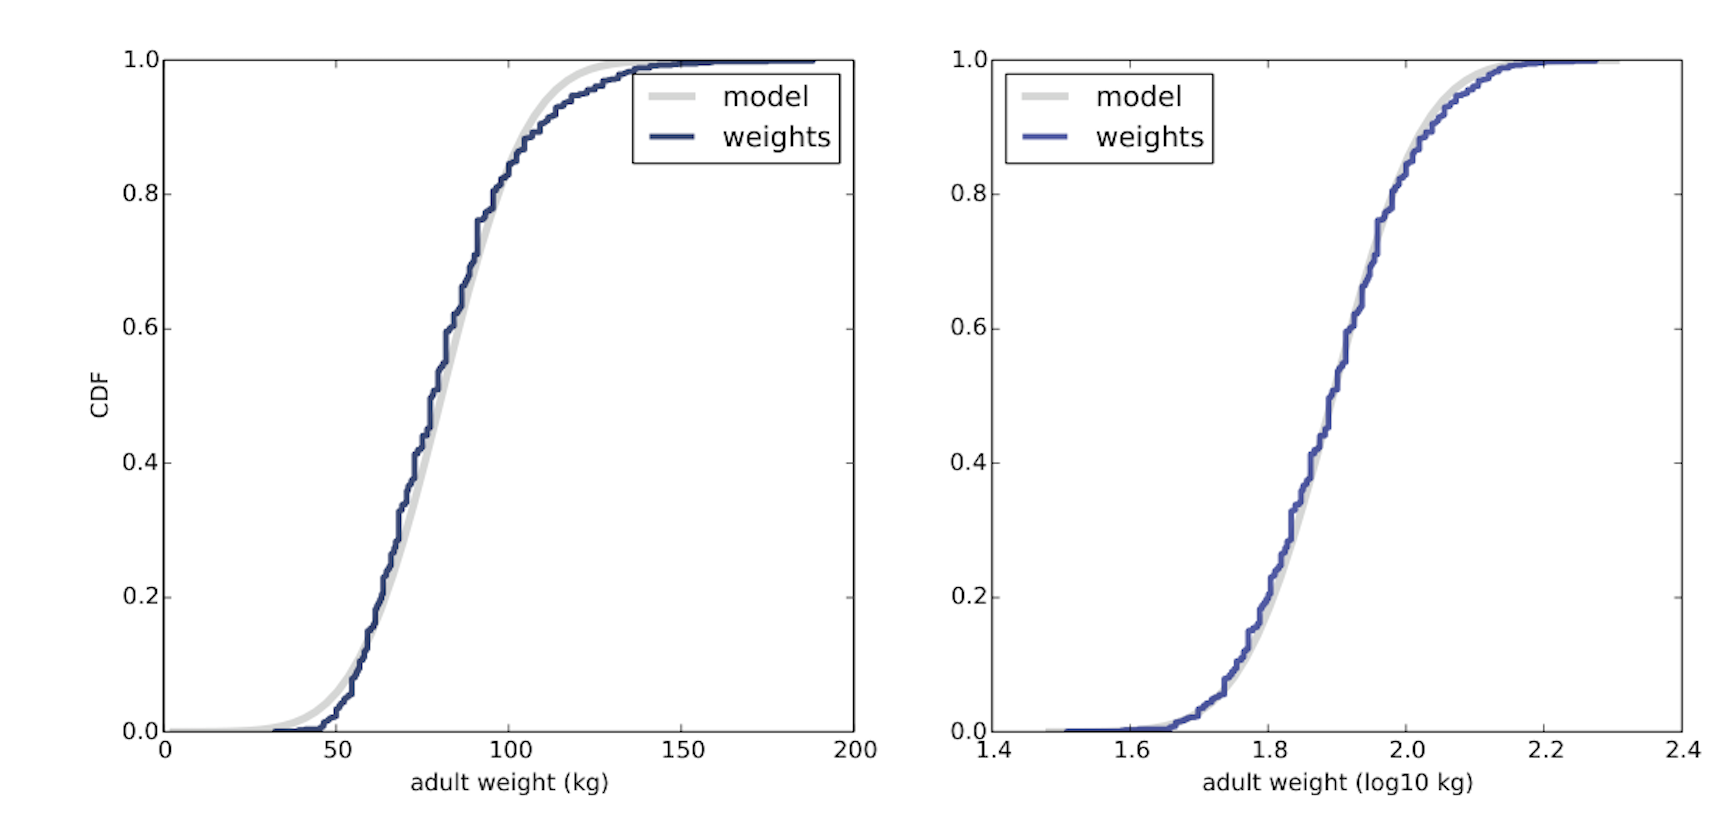
\includegraphics[width=\linewidth,height=0.6\textheight,keepaspectratio]{gfx/m2l2_thinkstats_fig5-7_adult_weights_linear_log_cdf.png}
\par\smallskip{\small \textbf{Hình 5.7:} CDF của cân nặng người lớn trên thang tuyến tính (trái) và thang log (phải).}
\end{figure}

...trong phạm vi một vài độ lệch chuẩn từ giá trị trung bình, nhưng không phải ở các phần đuôi. Liệu nó có đủ tốt cho các mục đích thực tế hay không phụ thuộc vào những mục đích đó.

\subsection*{5.4 Phân phối log-chuẩn}
\addcontentsline{toc}{subsection}{5.4 Phân phối log-chuẩn}

Nếu logarit của một tập hợp các giá trị có phân phối chuẩn, thì các giá trị đó có phân phối log-chuẩn (lognormal distribution). CDF của phân phối log-chuẩn giống với CDF của phân phối chuẩn, với $\log x$ được thay thế cho $x$.

$CDF_{lognormal}(x) = CDF_{normal}(\log x)$

Các tham số của phân phối log-chuẩn thường được ký hiệu là $\mu$ và $\sigma$. Nhưng hãy nhớ rằng các tham số này không phải là giá trị trung bình và độ lệch chuẩn; giá trị trung bình của một phân phối log-chuẩn là $\exp(\mu + \sigma^2/2)$ và độ lệch chuẩn của nó rất phức tạp (xem \url{http://wikipedia.org/wiki/Log-normal_distribution}).

Nếu một mẫu có phân phối xấp xỉ log-chuẩn và bạn vẽ CDF của nó trên thang đo $\log-x$, nó sẽ có hình dạng đặc trưng của một phân phối chuẩn. Để kiểm tra xem mẫu đó khớp với mô hình log-chuẩn tốt đến mức nào, bạn có thể tạo một biểu đồ xác suất chuẩn bằng cách sử dụng logarit của các giá trị trong mẫu.

% [PDF p.86 | in p.66]
\begin{figure}[H]
\centering
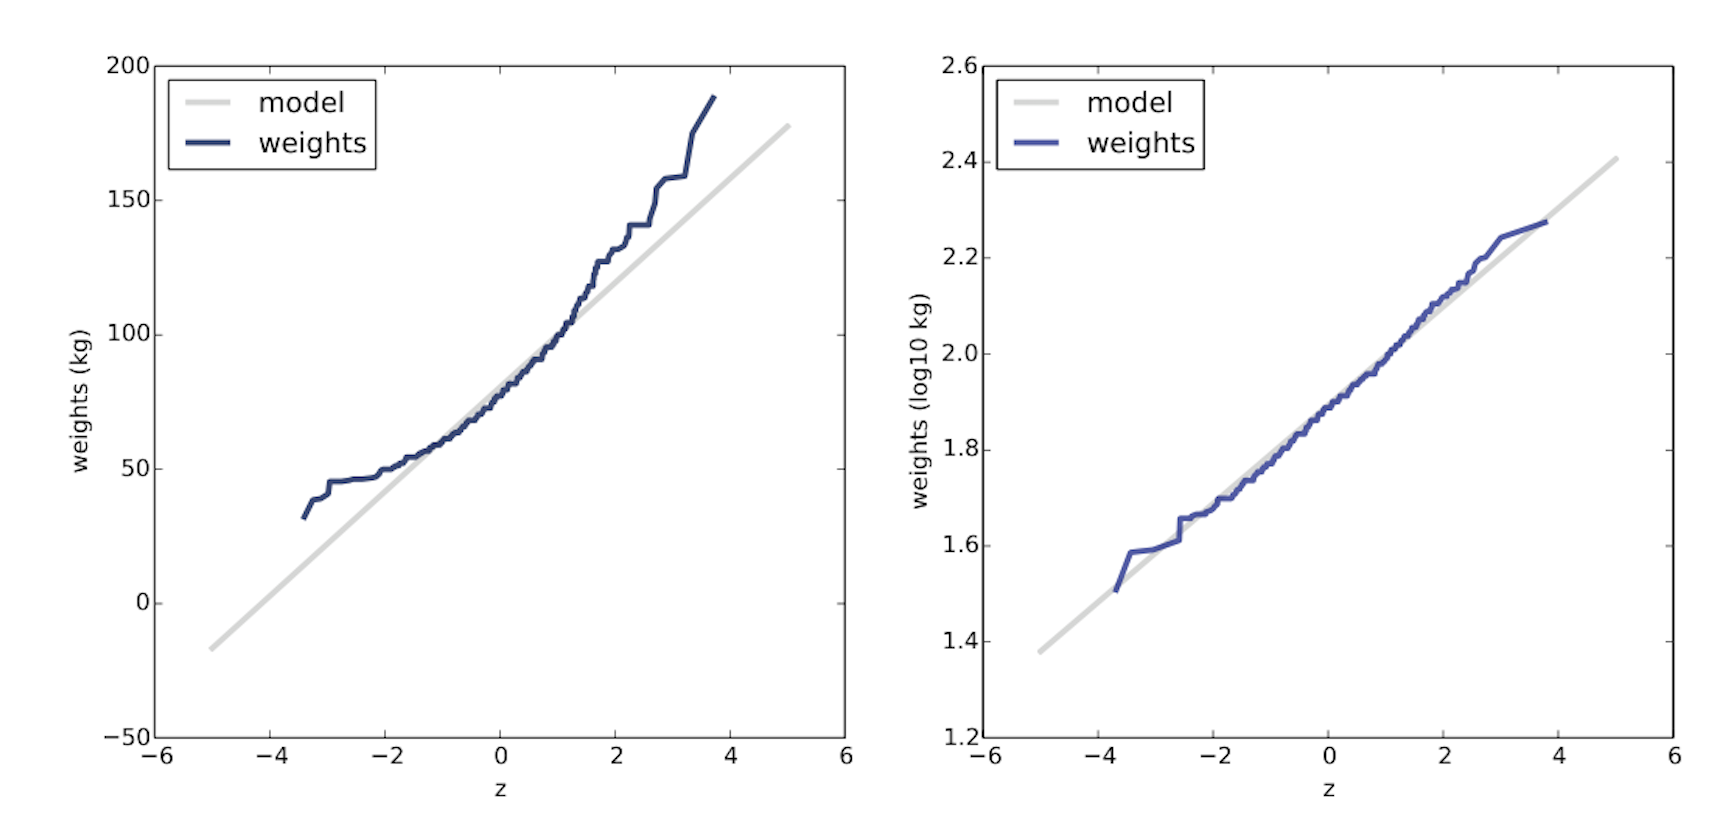
\includegraphics[width=\linewidth,height=0.6\textheight,keepaspectratio]{gfx/m2l2_thinkstats_fig5-8_adult_weights_linear_log_normal_plot.png}
\par\smallskip{\small \textbf{Hình 5.8:} Biểu đồ xác suất chuẩn cho cân nặng người lớn trên thang tuyến tính (trái) và thang log (phải).}
\end{figure}

Như một ví dụ, hãy xem xét phân phối cân nặng người lớn, có phân phối xấp xỉ log-chuẩn.$^2$

Trung tâm Ngăn ngừa Bệnh Mạn tính và Nâng cao Sức khỏe (National Center for Chronic Disease Prevention and Health Promotion) thực hiện một cuộc khảo sát hàng năm như một phần của Hệ thống Giám sát Yếu tố Nguy cơ Hành vi (Behavioral Risk Factor Surveillance System - BRFSS).$^3$ Năm 2008, họ đã phỏng vấn 414.509 người trả lời và hỏi về nhân khẩu học, sức khỏe và rủi ro sức khỏe của họ. Trong số dữ liệu họ thu thập được có cân nặng tính bằng kilogam của 398.484 người trả lời.

Kho lưu trữ cho cuốn sách này có chứa \texttt{CDBRFS08.ASC.gz}, một tệp ASCII có độ rộng cố định chứa dữ liệu từ BRFSS, và \texttt{brfss.py}, dùng để đọc tệp và phân tích dữ liệu.

Hình 5.7 (trái) cho thấy phân phối của cân nặng người lớn trên thang tuyến tính...

% [PDF p.87 | in p.67]
...với một mô hình chuẩn. Hình 5.7 (phải) cho thấy cùng một phân phối đó trên thang log với một mô hình log-chuẩn. Mô hình log-chuẩn phù hợp hơn, nhưng cách biểu diễn dữ liệu này không làm cho sự khác biệt trở nên quá rõ rệt.

Hình 5.8 cho thấy các biểu đồ xác suất chuẩn đối với cân nặng người lớn, $w$, và đối với logarit của chúng, $\log_{10} w$. Bây giờ có thể thấy rõ rằng dữ liệu sai lệch đáng kể so với mô hình chuẩn. Mặt khác, mô hình log-chuẩn là phù hợp tốt với dữ liệu.

$^2$ Tôi đã được mách nước về khả năng này bởi một bình luận (không có trích dẫn) tại \url{http://mathworld.wolfram.com/LogNormalDistribution.html}. Sau đó, tôi tìm thấy một bài báo đề xuất phép biến đổi logarit và gợi ý một nguyên nhân: Penman and Johnson, ``The Changing Shape of the Body Mass Index Distribution Curve in the Population,'' Preventing Chronic Disease, 2006 July; 3(3): A74. Trực tuyến tại \url{http://www.ncbi.nlm.nih.gov/pmc/articles/PMC1636707}.

$^3$ Centers for Disease Control and Prevention (CDC). Behavioral Risk Factor Surveillance System Survey Data. Atlanta, Georgia: U.S. Department of Health and Human Services, Centers for Disease Control and Prevention, 2008.
